\chapter{Úvod}
Cílem tohoto projektu je vytvořit elektronický budík s pokročilými funkcemi,
který lze snadno vyrobit v amatérských podmínkách a přizpůsobit tak, aby
vyhovoval i požadavkům náročného uživatele.

Zařízení není přímo připojené k síti Internet. Namísto toho bylo zvoleno
přípojení k serveru rozhraním UART. Server obsluhuje síťové funkce a poskytuje
například webové rozhraní, které umožňuje pohodlné nastavování časů a parametrů
buzení. Budík lze plně využívat i bez serveru. Server tak ani nemusí běžet po
celý den, lze použít běžný osobní počítač. Vhodnou volbou serveru pro
nepřetržitý provoz je nepříklad jednodeskový počítač Raspberry Pi.

Zdrojový kód firmware a serverového software, schéma zapojení, návrh desky
plošných spojů i 3D model krabičky jsou uvolněny pod svobodnou
licencí MIT\footnote{\url{https://cs.wikipedia.org/wiki/Licence_MIT}}.
Projekt tak vyhovuje filozofii svobodného
software\footnote{\url{https://www.gnu.org/philosophy/free-sw.html}}
a open-source
hardware\footnote{\url{https://cs.wikipedia.org/wiki/Open-source_hardware}}.

Zdrojový kód firmware je opatřed komentáři, z nichž je generována dokumentace
pomocí nástroje \shellcmd{doxygen}. To usnadňuje orientaci v projektu
a umožňuje, aby si i běžný uživatel se základní znalostí programování
implementoval dodatečné funkce, které potřebuje.

Budík je zařízení, jehož selhání může uživateli způsobit problémy a v některých
případech i finanční škodu. Velká pozornost je proto věnována zajištění
spolehlivosti. Nechtěné vzbuzení uživatele například při výpadku napájení je
přitom upřednosťnováno před rizikem nevzbuzení. Preventivní opatření jsou
uplatněna jak na úrovni firmware (aktivace časovače \acs{WDT}, automatické
testy), tak i na úrovni hardware (použití antistatického vybavení při osazování
desky plošných spojů).

\paragraph{Motivace}
Mnoho požadavků na funkce budíku vychází ze zkušenosti s komerčně dostupnými
řešeními. Autor této práce po několik let používal radiobudík Sencor
SRC~330~GN. Během jeho užívání bylo odhaleno několik problému, především
nedostatek nastavitelných časů buzení (pouze 2), nemožnost přiřadit budicímu
času libovolnou skupinu dní v týdnu a problémy se zrušením budíku v průběhu
odložení pomocí funkce \uv{snooze}. Nepříjemná byla také chyba ve firmware,
která se projevovala nepřerušitelným pískáním, ke kterému docházelo náhodně
v první hodině po stisku tlačítka nastavujícího dobu nečinnosti, po které dojde
ke zhasnutí displeje. Protože tento komerčně dostupný budík neumožňuje zásah
uživatele do firmware, neexistuje žádná možnost, jak tyto nedostatky odstranit.
Mezi další problémy patřilo i slyšitelné bzučení o frekvenci \SI{50}{\hertz}
vydávané interním transformátorem (zařízení je napájeno síťovým napětím).

\begin{figure}[htbp]
    \centering
    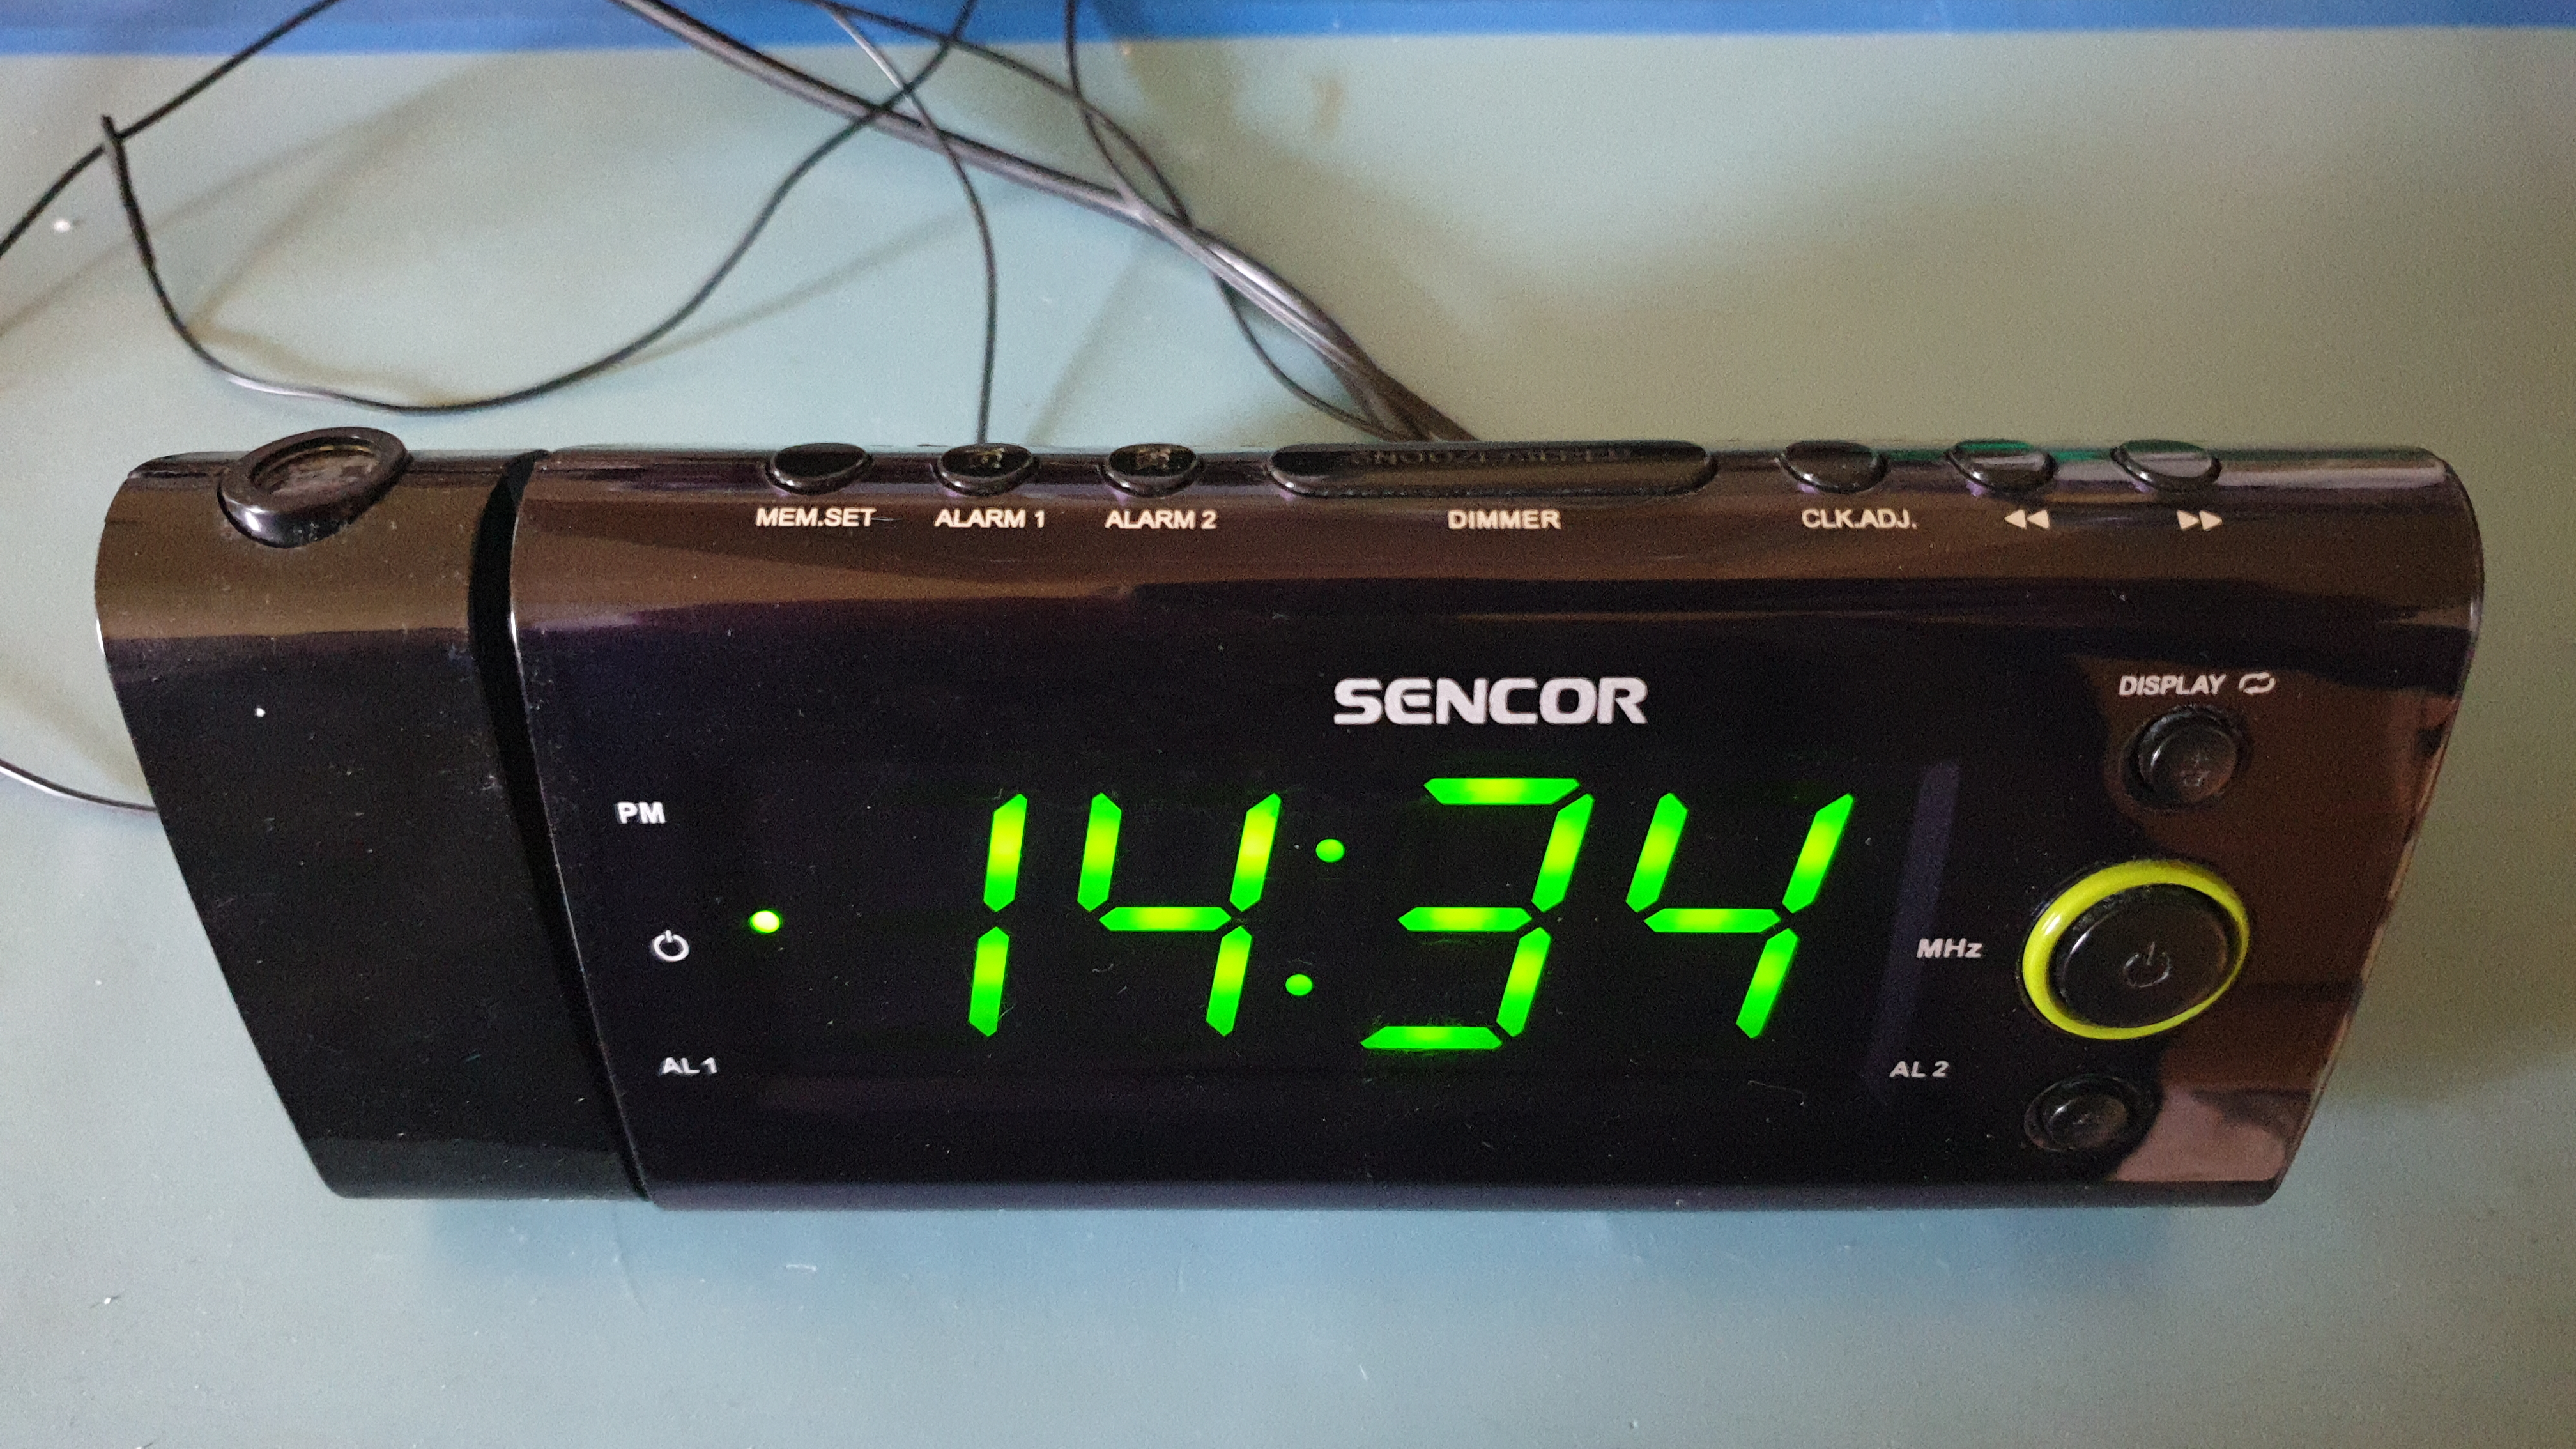
\includegraphics[width=0.8\textwidth]{sencor-SRC-330-GN}
    \caption{Komečně dostupný budík Sencor SRC~330~GN}
    \label{fig:sencor}
\end{figure}


\paragraph{Struktura práce}
Práce je členěna do kapitol (viz \hyperref[toc]{Obsah}). První kapitola se
věnuje hardwarové části výrobku a programu, který běží na jeho mikrokontroléru
(firmware). Druhá kapitola se věnuje software, tedy programům bežícím na
serveru.

Samostatné celky (zdrojové kódy firmware, software, návrh hardware) jsou
umístěny v oddělených repozitářích systému \shellcmd{git}. V repozitáři se
zdrojovými kódy této práce jsou ale všechny části vloženy jako submoduly
v adresáři \repopath{prilohy/}. Více informací o členění elektronické přílohy
práce lze nalézt v příloze~\vref{app:dirtree}.

Dokument obsahuje výpisy jednoduchých programů a ukázky zdrojového kódu.
Ty jsou otištěny v polích ohraničených rámečkem. Je využito písmo s pevnou
šířkou (neproporcionální písmo). Pro různé programovací jazyky jsou využívány
vhodné zvýrazňovače syntaxe. Příliš dlouhé řádky jsou zalamovány, pokračování
zalomeného řádku je označeno symbolem \lstpostbreak{}.

\begin{lstlisting}[language=hashcomment]
Toho je ukázkový výpis.
Běžný text.
# komentář
Další Řádek.
Tento text je tak dlouhý, že se nevejde na jeden řádek a musí být zalomen, přičemž jeho pokračování je jasně označeno.
Další Řádek.
\end{lstlisting}

Řádky delších úplných výpisů jsou číslovány:
\begin{lstlisting}[language=hashcomment,style=numbers]
Toho je ukázkový výpis.
Běžný text.
# komentář
Další Řádek.
Tento text je tak dlouhý, že se nevejde na jeden řádek a musí být zalomen, přičemž jeho pokračování je jasně označeno.
Další Řádek.
\end{lstlisting}

Při práci s programy pro příkazový řádek je využíván unixový shell.
Text zkopírovaný z terminálu je tisknut následujícím stylem:
\begin{lstlisting}[style=terminal]
$ lsb_release -a 2>/dev/null | pr -Td | cowsay -f tux
 _________________________________
/ Distributor ID: Ubuntu          \
|                                 |
| Description: Ubuntu 20.04.4 LTS |
|                                 |
| Release: 20.04                  |
|                                 |
\ Codename: focal                 /
 ---------------------------------
   \
    \
        .--.
       |o_o |
       |:_/ |
      //   \ \
     (|     | )
    /'\_   _/`\
    \___)=(___/

$
\end{lstlisting}
Řádky začínající znakem \texttt{\$} obsahují zadávaný příkaz, na následujících
řádcích je jeho textový výstup.
